\documentclass[tikz]{standalone}
\usepackage{pgfplots, pgfplotstable, booktabs,ifthen,hyperref}
\usepackage{sqrcaps}
\renewcommand{\arraystretch}{1.25}
\setlength{\tabcolsep}{12pt}

\tikzstyle{block}=[black, ultra thick, rounded corners, minimum width=2cm, minimum height=2cm, anchor= north west, fill=white, fill opacity = 0.8, text opacity =1, font=\bf]

\begin{document}
\begin{tikzpicture}
	\clip (0,0) rectangle (8.5in, 11in);
	\node[inner sep=0pt, outer sep=0pt, anchor=south west, opacity=0.5] at (0,0) {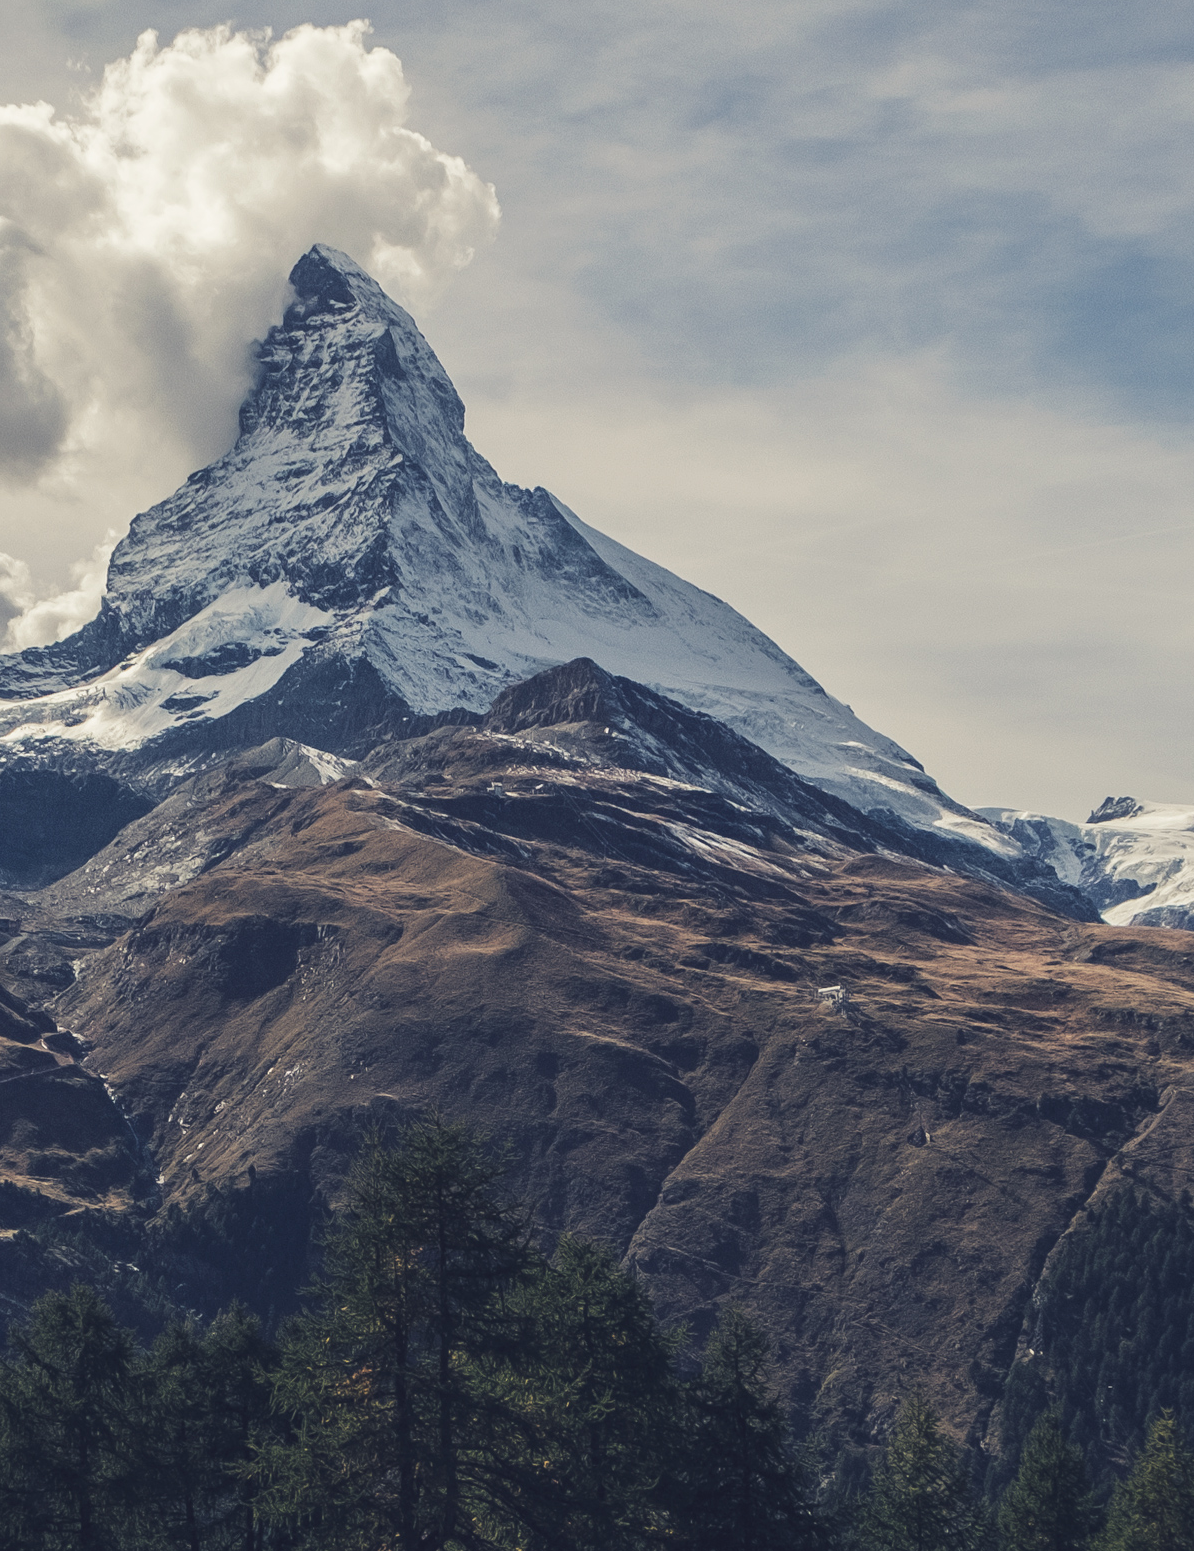
\includegraphics[width=8.5in]{mountain.png}};

	\node[block, minimum width=7cm,font=\LARGE] at (5in,9.5in) {
	  \pgfplotstabletypeset[ col sep = comma,
		every head row/.style = {output empty row},
		columns/Name/.style={string type, column type=l|},
		columns/Rating/.style={dec sep align},
		%every last row/.style={before row = \midrule},
		] {../results.csv}
	  };

	  \node[font=\Huge,align=left,anchor=north west] at (1cm,10.5in) {\sqrcfamily Digital Dodgeball\\\sqrcfamily Leaderboards};

	  \node[inner sep=0pt, outer sep=0pt, anchor=south west] at (1cm,1cm) {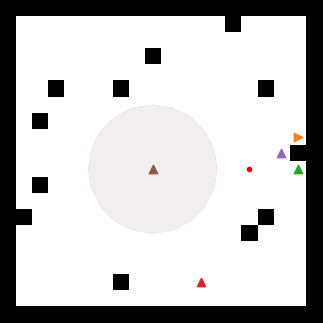
\includegraphics[width=4in]{anim.png}};

	  \node[block, minimum width=5cm, font=\Large, text width=7cm, align=center] at (5in,6.5cm) {Rankings as of October 27};

	  \node[block, minimum width=5cm, font=\Large, text width=7cm, align=center, anchor=south west] at (5in,1cm) {Interested in joining!? Contact $\langle$jjrembold$\rangle$ or visit \nolinkurl{github.com/jrembold/WUPhys-CodeComp} to join the fun! All are welcome!};
\end{tikzpicture}

\end{document}
